\documentclass{beamer}
\usepackage{graphicx}
\usepackage{paralist}
\usepackage{outlines}

\title{Selection Tools}
\author{Mendocino College - DAM 110}
\titlegraphic{\vspace{-10mm}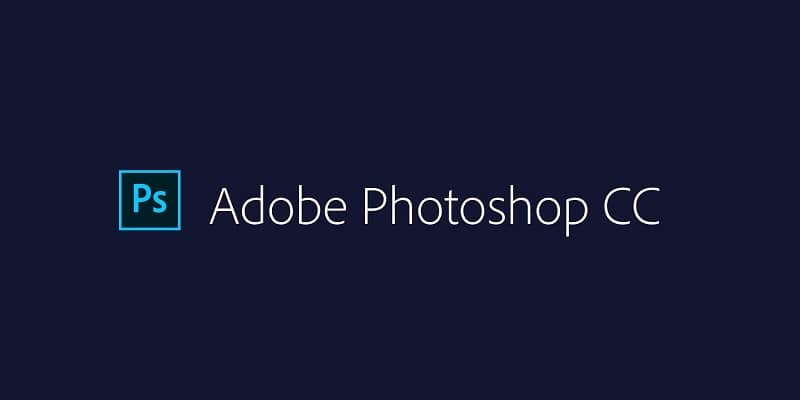
\includegraphics[width = .8\textwidth]{images/photoshop.jpg}} 
\date{\vspace{-5em}} 


\mode <presentation>
\usetheme{Warsaw}
\usecolortheme{default}

\setbeamerfont{footline}{size=\fontsize{5}{8}\selectfont}

\definecolor{darkred}{rgb}{20,0,0}
\definecolor{darkgreen}{RGB}{40,110,20}
\definecolor{darkpurple}{RGB}{30,0,30}
\definecolor{chardonnay}{RGB}{255, 255, 204}

\setbeamercolor*{palette primary}{fg=white, bg=darkgreen}


\begin{document}
	{
		\setbeamertemplate{footline}{} 
		\setbeamertemplate{headline}{} 
		\begin{frame}
			\vspace{-35pt}
			\maketitle
		\end{frame}
	}



	\section{What are the Selection Tools?}
		\begin{frame}
		\frametitle{Selection Tools}
		\begin{center}
			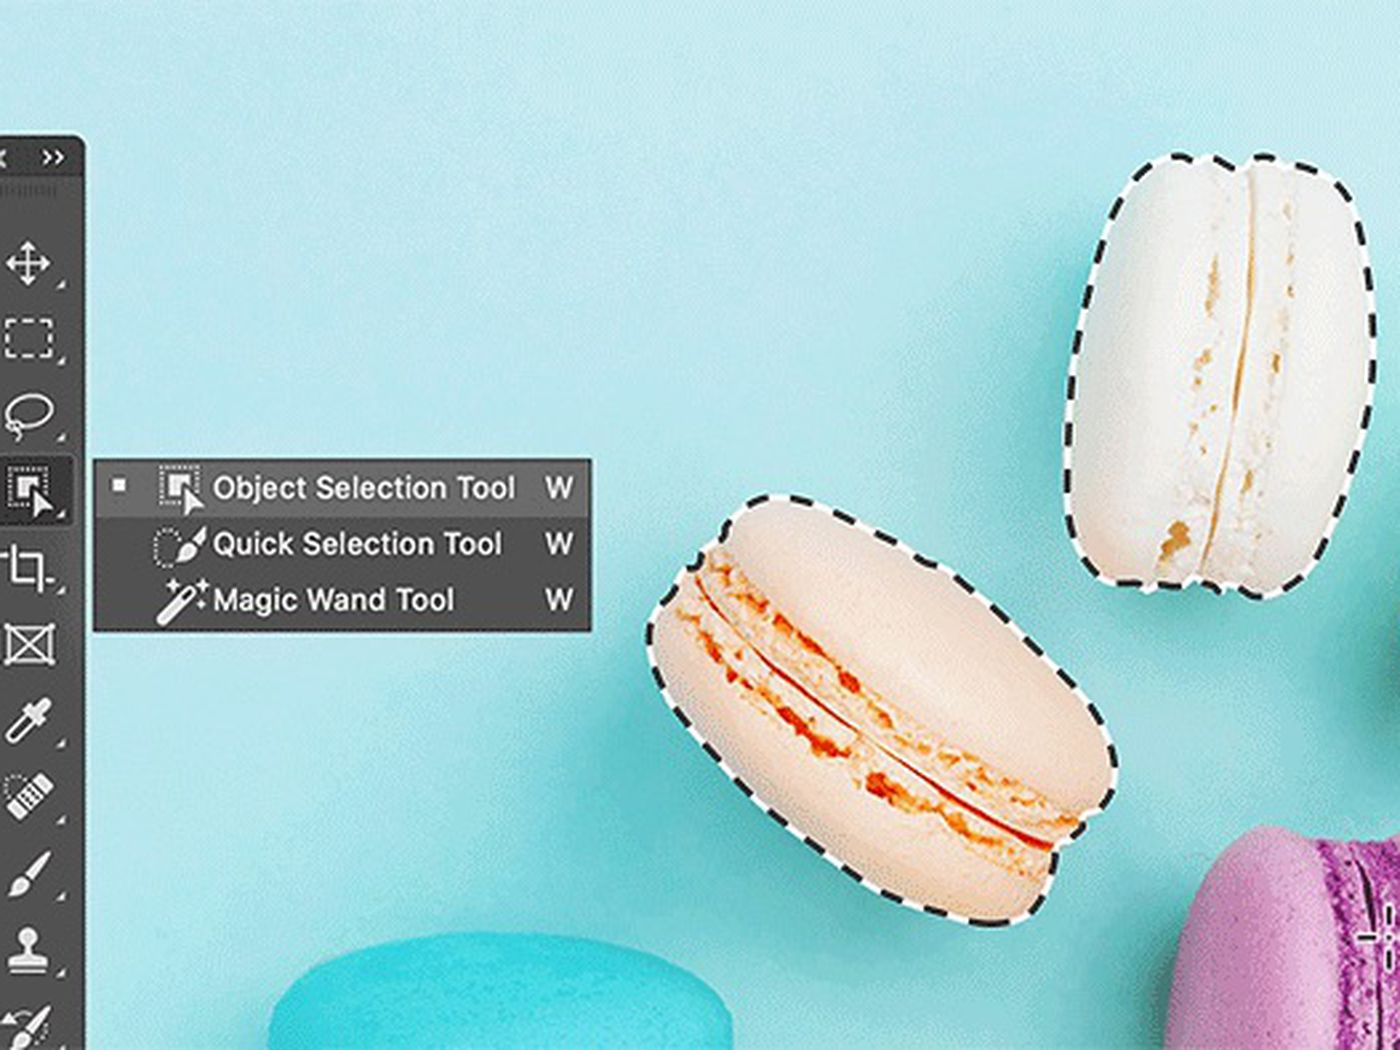
\includegraphics[width = 0.8\textwidth]{images/Photoshop_10_56.jpg}
		\end{center}
	\end{frame}
	
			\subsection{What are Selection Tools?}		
	\begin{frame}
		\frametitle{What are Selection Tools?}
	\begin{outline}
		\1 A selection isolates part of an image so you can work on that area without affecting the rest of the image.
		\1 By selecting specific areas, you can edit and apply effects and filters to portions of your image while leaving the unselected areas untouched.
		\1 When you make a selection, a border appears around the selection area. 
		\1 You can move, copy, or delete pixels inside the selection border, but you can’t touch areas outside the selection border until you deselect the selection. 
		\2 You can deselect by pressing Ctrl + D
	\end{outline}
\begin{center}
	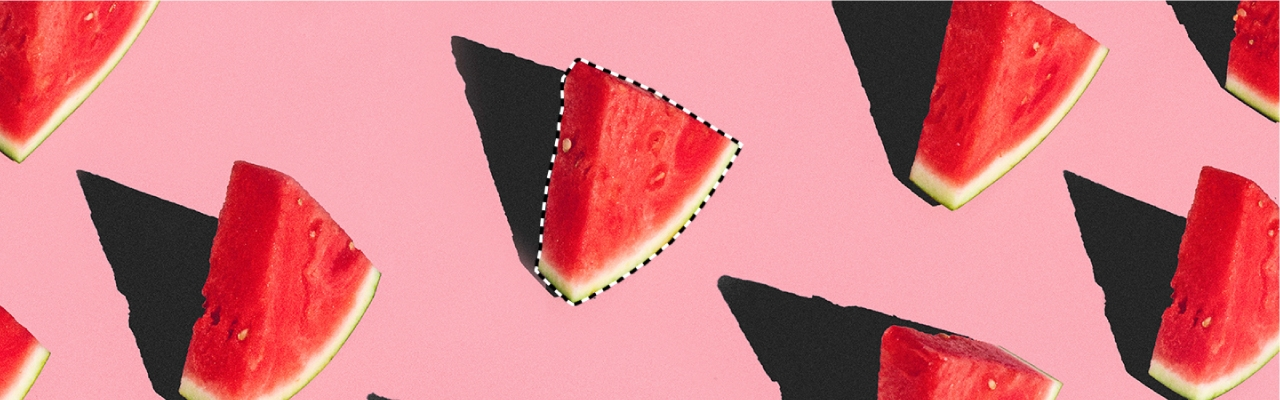
\includegraphics[width=.7\textwidth]{images/whats-new-detail-auto-select-an-object-on-hover-ps-23.0-max-oct2021.jpg.img.jpg}
	\end{center}
		\end{frame}

	
	\section{Quick Selection Tools}
	\begin{frame}
		\frametitle{Quick Selection Tools}
		\begin{center}
			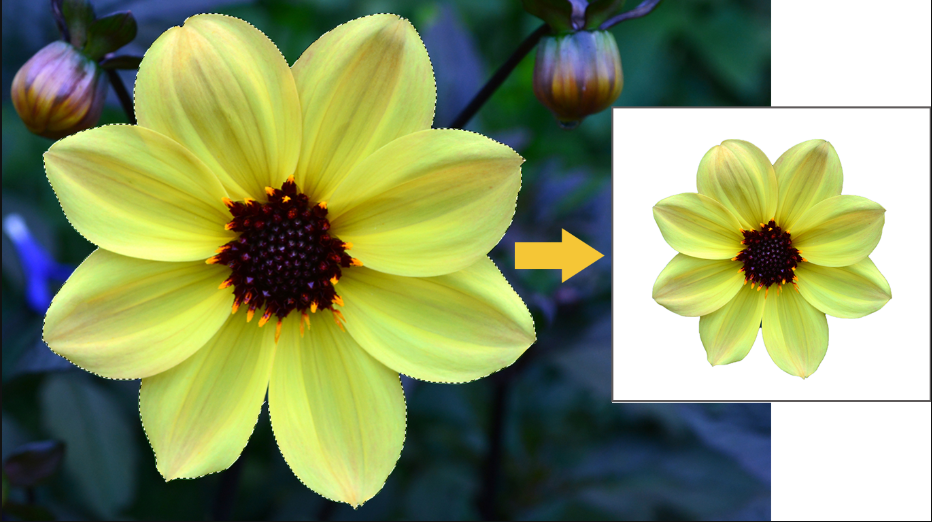
\includegraphics[width = 1.0\textwidth]{images/selection1.png}
		\end{center}
	\end{frame}

\subsection{Quick Selection Tool}
\begin{frame}
	\frametitle{Quick Selection Tool}
	\begin{outline}
		\1 The Quick Selection tool  to quickly "paint" a selection using an adjustable round brush tip. 
		\1 As you drag, the selection expands outward and automatically finds and follows defined edges in the image.
		\1 Paint inside the part of the image you want to select. The selection grows as you paint. 
		\2 As you paint near the edges of a shape, the selection area extends to follow the contours of the shape edge.
	\end{outline}
	\begin{center}
		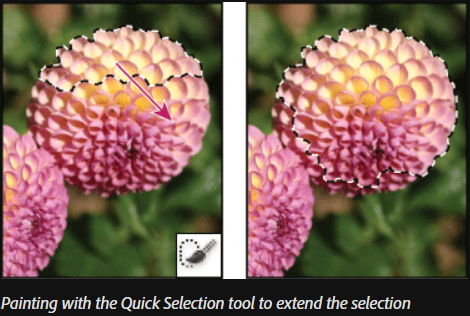
\includegraphics[width = 0.75\textwidth]{images/quick select.png}
	\end{center}
\end{frame}

\begin{frame}
	\frametitle{Quick Selection Tool - Options}
	\begin{outline}
		\1 Sample All Layers: 
		\2 Creates a selection based on all layers instead of just the currently selected layer.
		\1 Enhance Edge: 
		\2 Reduces roughness and blockiness in the selection boundary. Enhance Edge automatically flows the selection further toward image edges and applies some of the edge refinement you can apply manually in the Select and Mask workspace.
		\1 To subtract from a selection, click the Subtract From option in the options bar, then drag over the existing selection.
		\2 To temporarily switch between add and subtract modes, hold down the Alt key.
	\end{outline}
	\begin{center}
		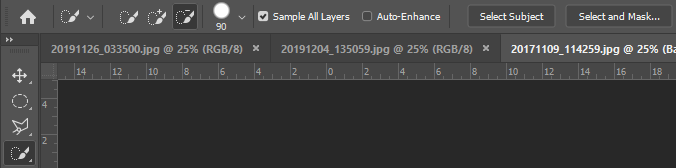
\includegraphics[width = 0.8\textwidth]{images/quick select options.png}
	\end{center}
\end{frame}

	
\subsection{Magic Wand Tool}
\begin{frame}
	\frametitle{Magic Wand Tool}
	\begin{outline}
		\1 The Magic Wand tool lets you select a consistently colored area (for example, a red flower) without having to trace its outline. 
		\1 You specify the selected color range, or tolerance, relative to the original color you click.
		\1 You cannot use the Magic Wand tool on an image in Bitmap mode or on 32‑bits-per-channel images.
	\end{outline}
	\begin{center}
		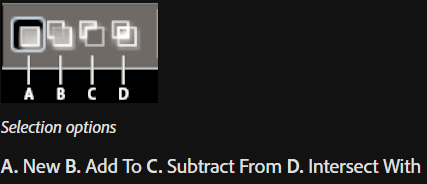
\includegraphics[width = 0.9\textwidth]{images/magic wand1.png}
	\end{center}
\end{frame}

\begin{frame}
	\frametitle{Magic Wand Tool - Options}
	\begin{outline}
		\1 Tolerance: 
		\2 Determines the color range of selected pixels. Enter a value in pixels, ranging from 0 to 255. A low value selects the few colors very similar to the pixel you click. A higher value selects a broader range of colors.
		\1 Anti-aliased: 
		\2 Creates a smoother-edged selection.
		\1 Contiguous: 
		\2 Selects only adjacent areas using the same colors. Otherwise, all pixels in the entire image using the same colors are selected.
		\1 Sample All Layers: 
		\2 Selects colors using data from all the visible layers. Otherwise, the Magic Wand tool selects colors from the active layer only.
	\end{outline}
	\begin{center}
		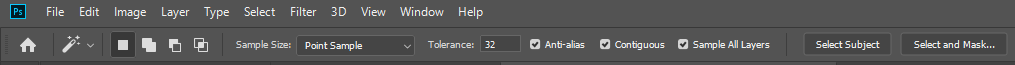
\includegraphics[width = 1.1\textwidth]{images/magic wand2.png}
	\end{center}
\end{frame}


\subsection{Object Selection Tool}
\begin{frame}
	\frametitle{Object Selection Tool}
	\begin{outline}
		\1 Released in June 2022, this selection tool is not available to us in the classroom.
		\1 It is available at the computers in the Coast Center
		\2 But we will not be using it this class.  
		\1 The Object Selection tool simplifies the process of selecting a single object or part of an object in an image—people, cars, furniture, pets, clothes, and more. You can simply draw a rectangular region or a lasso around the object and let the Object Selection tool automatically select the object inside the defined region. Selections made with the Object Selection tool are now more accurate and preserve more details in the edges of the selection, which means you spend less time getting those perfect selections.
	\end{outline}
\end{frame}

\section{Fine Tuning Your Selected Areas}
\subsection{Inverting Your Selection}
\begin{frame}
	\frametitle{Inverting Your Selection}
	\begin{outline}
		\1 To select everything else outside of what you selected, you can invert your selected area.
		\1 From the Menu Bar:  Select - Inverse
		\1 Keyboard Shortcut:  Ctrl + Shift + I
	\end{outline}
	\begin{center}
		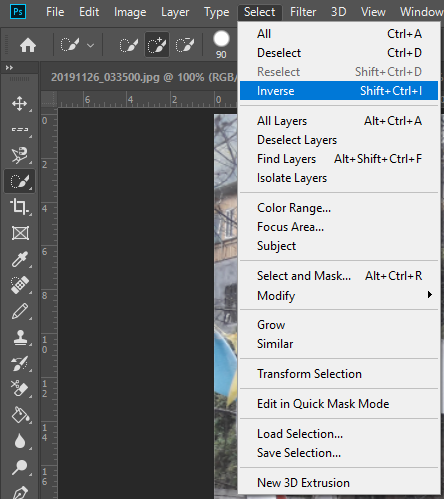
\includegraphics[width = 0.7\textwidth]{images/invert selection.png}
	\end{center}
\end{frame}

\subsection{Fine Tuning Your Selected Areas}
\begin{frame}
	\frametitle{Fine Tuning Your Selected Areas}
	\begin{outline}
		\1 The Quick Selection Tools can do a tremendous amount of work for you,
		\2 But it is still just a machine guessing based on the shades of the pixels next to each other.
		\1 To select an area perfectly will require using multiple selection tools.
		\1 So now we will be presenting the other selection tools available to us.
	\end{outline}
	\begin{center}
		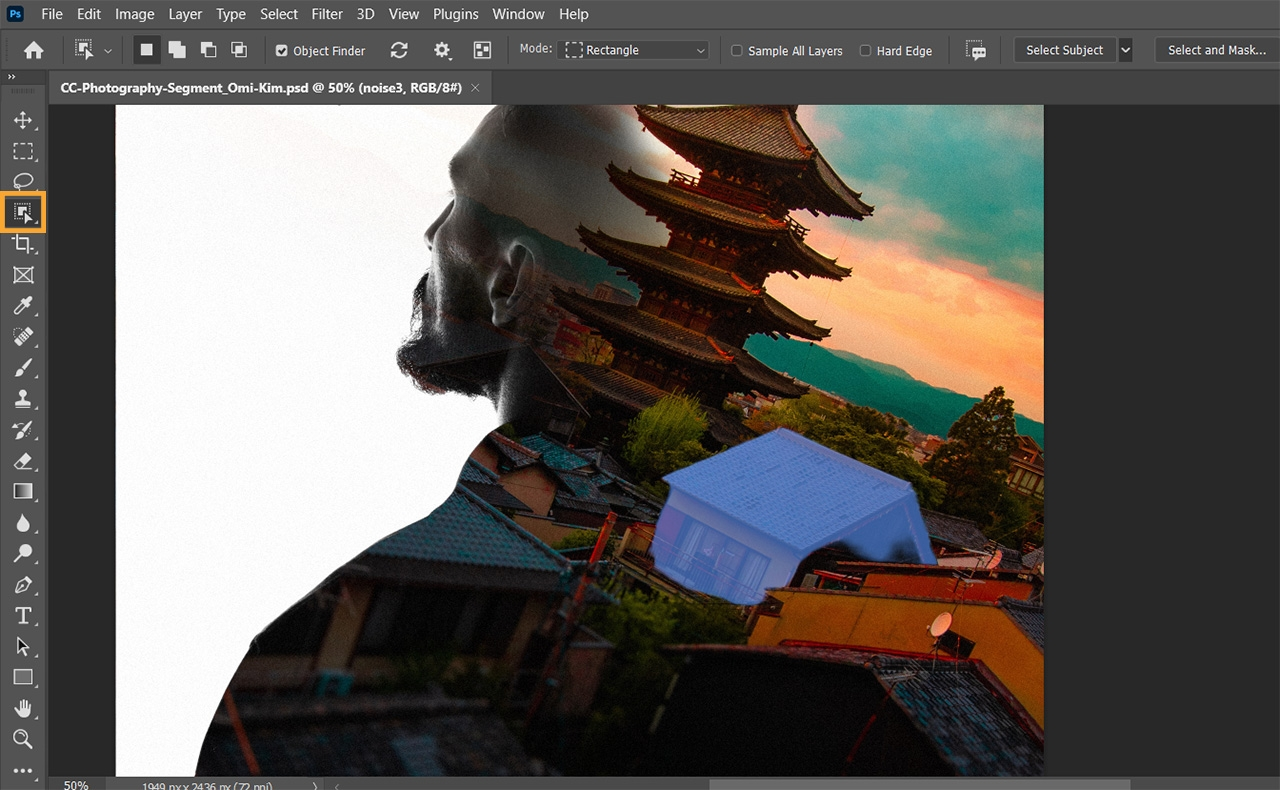
\includegraphics[width = 0.7\textwidth]{images/ps-object-selection-on-hover.jpg.img.jpg}
	\end{center}
\end{frame}

\end{document}